\documentclass{article}
\usepackage{otherpreamble}
\usepackage{env}
\usepackage{configure}

\graphicspath{ {./figures/} }

% available environments:
% theorem: thm
% definition: defn
% proof: pf
% corollary: crll
% lemma: lm
% question: qu
% solution: soln
% example: xmp
% exercise: exr
%
% options: title=<title>   {all}
%          source=<source> {pf, qu, soln, xmp, exr}  Note: if content is taken directly from the main resource, cite the main resource as ``Primary source material"


% define these variables!
\def\coursecode{}
\def\coursename{} % use \relax for non-course stuff
\def\studytype{} % 1: Personal Self-Study Notes / 2: Course Lecture Notes / 3: Revised Notes / 4: Exercise Solution Sheet
\def\author{\me}
\def\createdate{October 18, 2024}
% \def\updatedate{\today}
\def\source{\relax} % name, ed. of textbook, or `Class Lectures` for class notes
\def\sourceauthor{\relax} % for class notes, put lecturer
% \def\leftmark{} % set text in header; should only be necessary in assignments etc.
% \pagenumbering{arabic} % force revert numbering to default; should only be necessary in assignments etc.

\begin{document}

\cover
\toc
\pagenumbering{arabic}

% start here

\newpage
\section{Overview of Sokoban}

This section will give a brief overview of the game Sokoban and its rules.

Sokoban is a puzzle game, where the objective of the player is to push boxes into target positions.
The arena is depicted as a square grid, although the playable area does not necessarily have to
constitute a square.

The player can move either horizontally or vertically, one tile at a time, and cannot move through
boxes or walls. The player can push boxes by standing next to a box and moving in the direction they
wish to push the box. Boxes cannot be pushed onto tiles containing a wall or another box; only one
box may be pushed at a time. Furthermore, boxes cannot be pulled.

The number of boxes always matches the number of target positions.
The puzzle is solved when all boxes are moved onto all target positions.
Each arena is randomly generated in such a way that a solution always exists.

\newpage
\section{Using CPUlator}

This guide will begin by explaining how to load the game using CPUlator.
It is assumed that you (the reader of this guide) have already downloaded
the relevant \texttt{game.s} game file.

\subsection{Opening CPUlator}

CPUlator is a website which allows a user to execute assembly code.
This game has been written using the RISC-V RV32 SPIM formatting.

To begin, open CPUlator by clicking the following link:
\begin{center}
    \href{https://cpulator.01xz.net/?sys=rv32-spim}{https://cpulator.01xz.net/?sys=rv32-spim}
\end{center}
You should be greeted with a screen similar to the following in Figure 1:
\begin{figure}[ht]
    \centering
    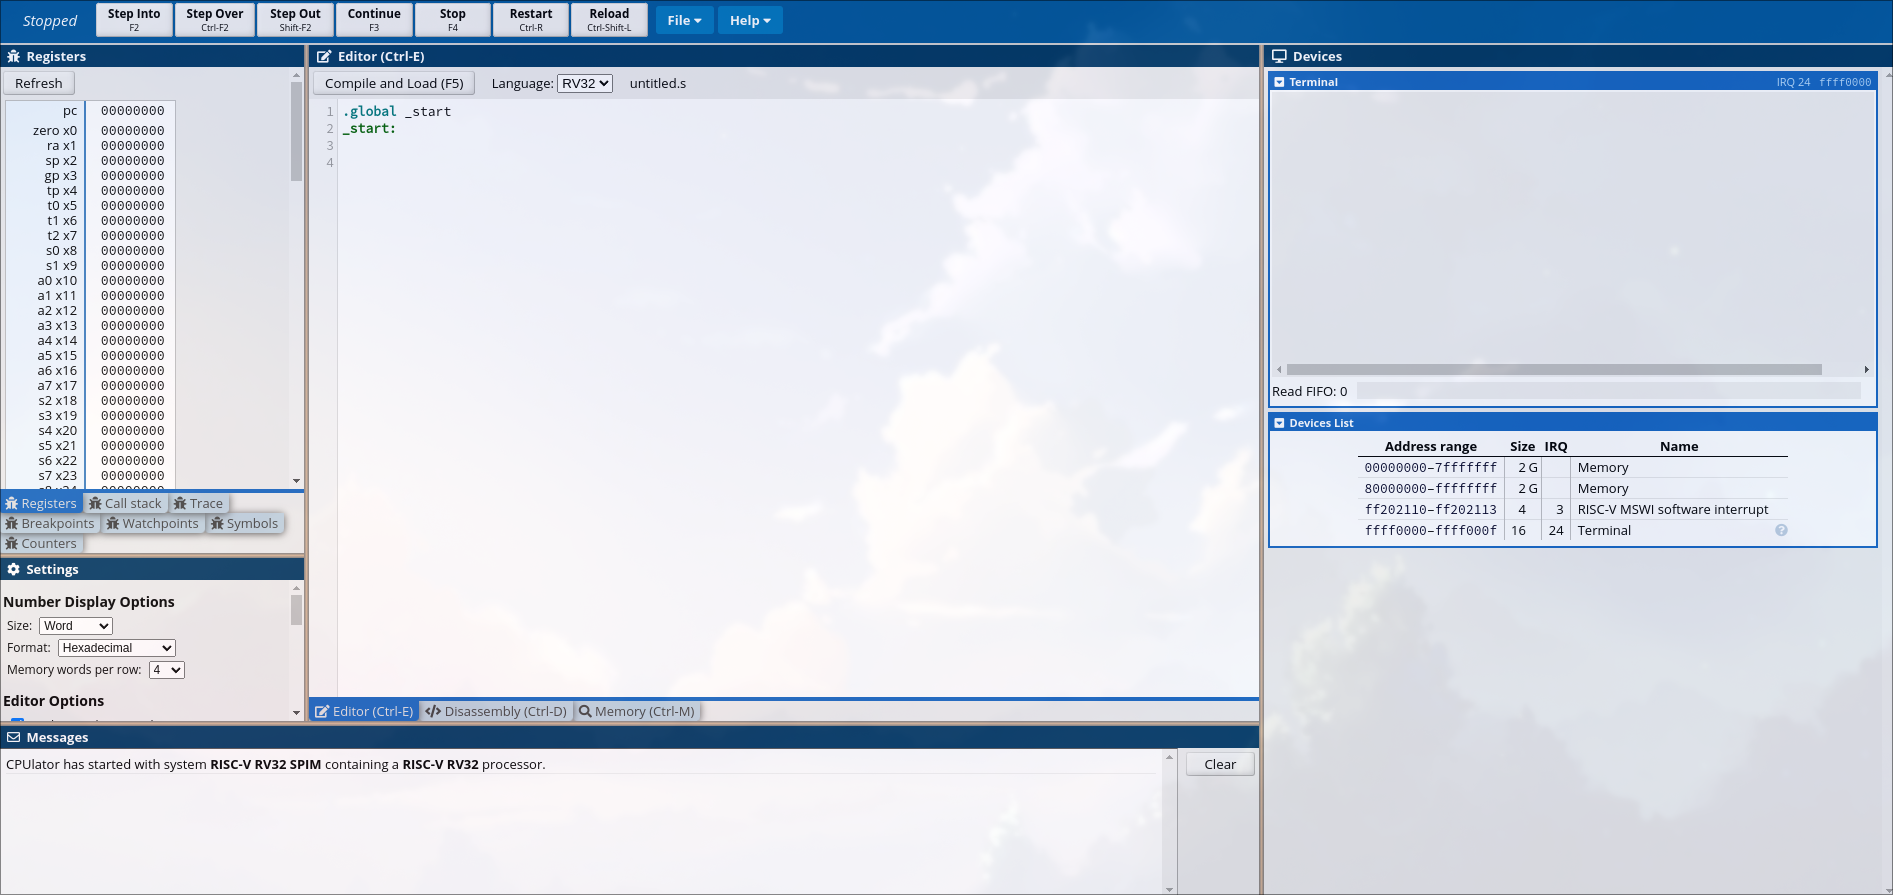
\includegraphics[width=0.7\linewidth]{mainscreen}
    \caption{The main interface of CPUlator}
\end{figure}

Alternatively, the website can be visited directly.
If the website is opened manually, there are a few extra steps necessary.

Rather than seeing the screen shown in Figure 1, you likely see what's in Figure 2.

\begin{figure}[ht]
    \centering
    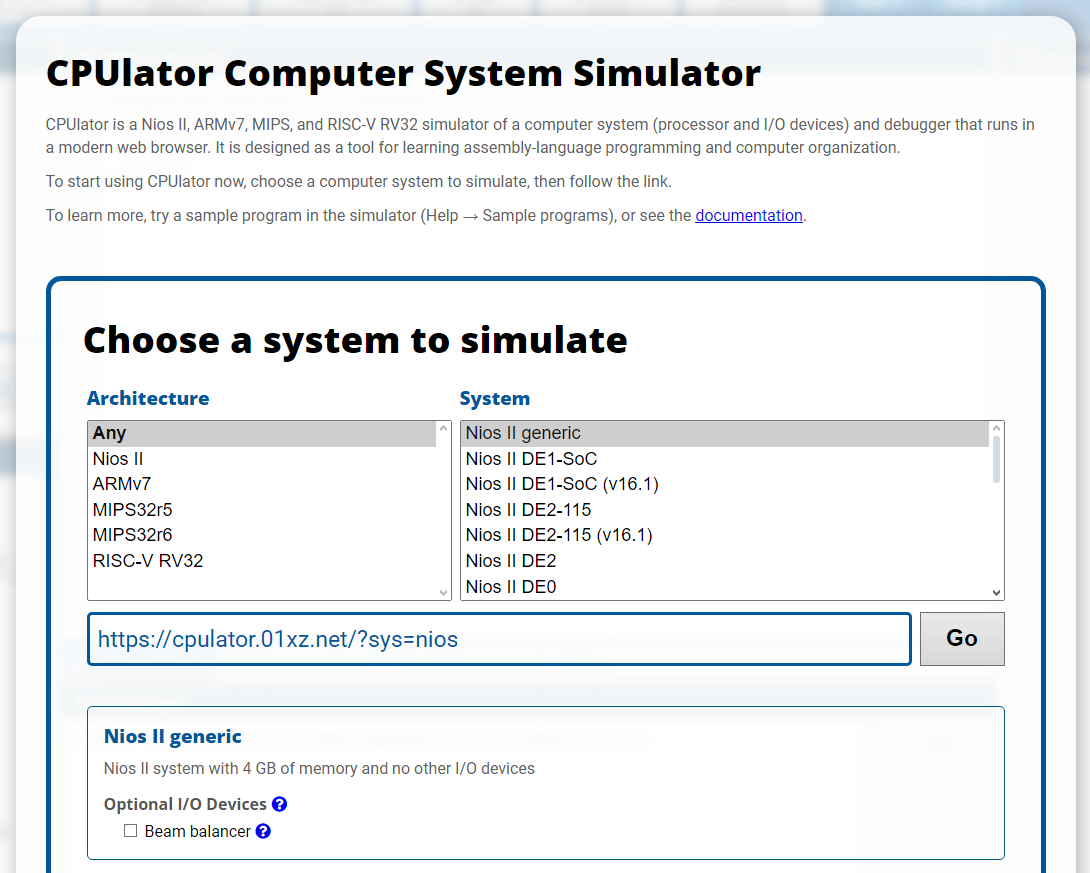
\includegraphics[width=0.5\linewidth]{default}
    \caption{The default interface when opening CPUlator without settings}
\end{figure}

\newpage
If this is the case, under the ``Architecture" column,
click on the option labelled ``RISC-V RV32" (outlined in red in Figure 3).

\begin{figure}[ht]
    \centering
    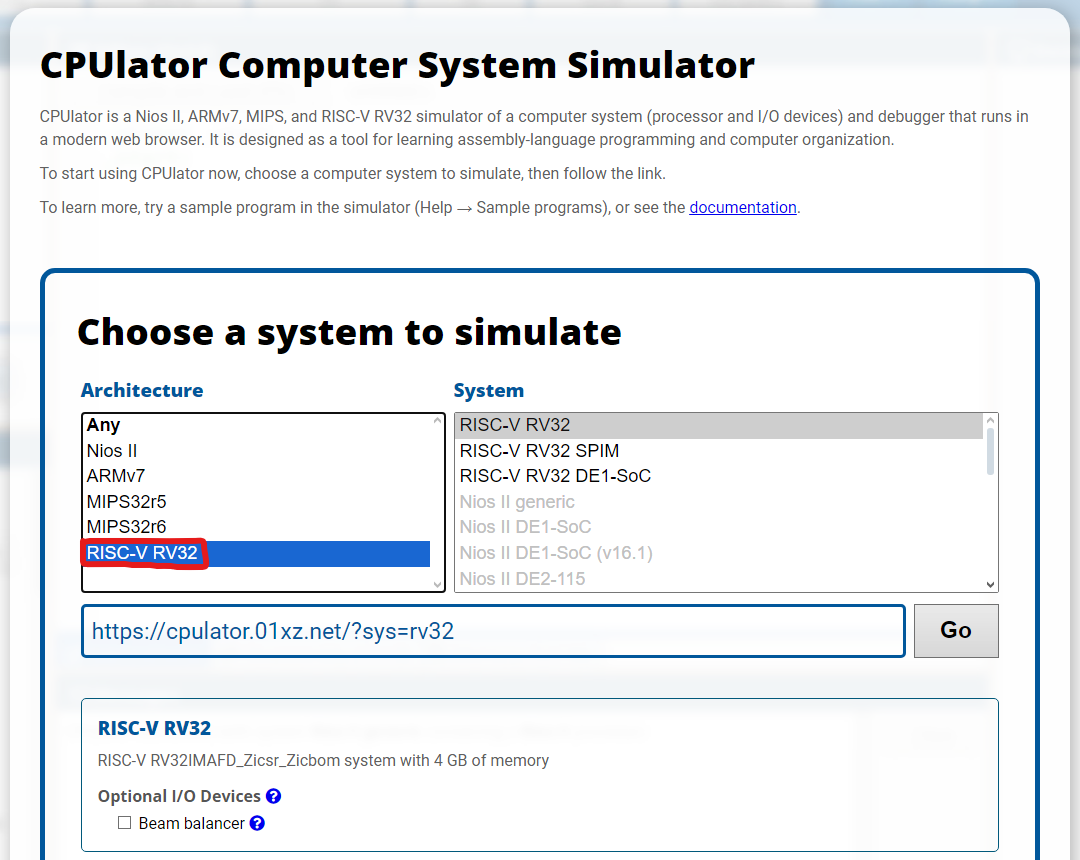
\includegraphics[width=0.5\linewidth]{riscv}
    \caption{The RISC-V RV32 option}
\end{figure}

Then, click the ``RISC-V RV32 SPIM" option under the ``System" column
(outlined in red in Figure 4), and click the ``Go" button (outlined in green in Figure 4).

\begin{figure}[ht]
    \centering
    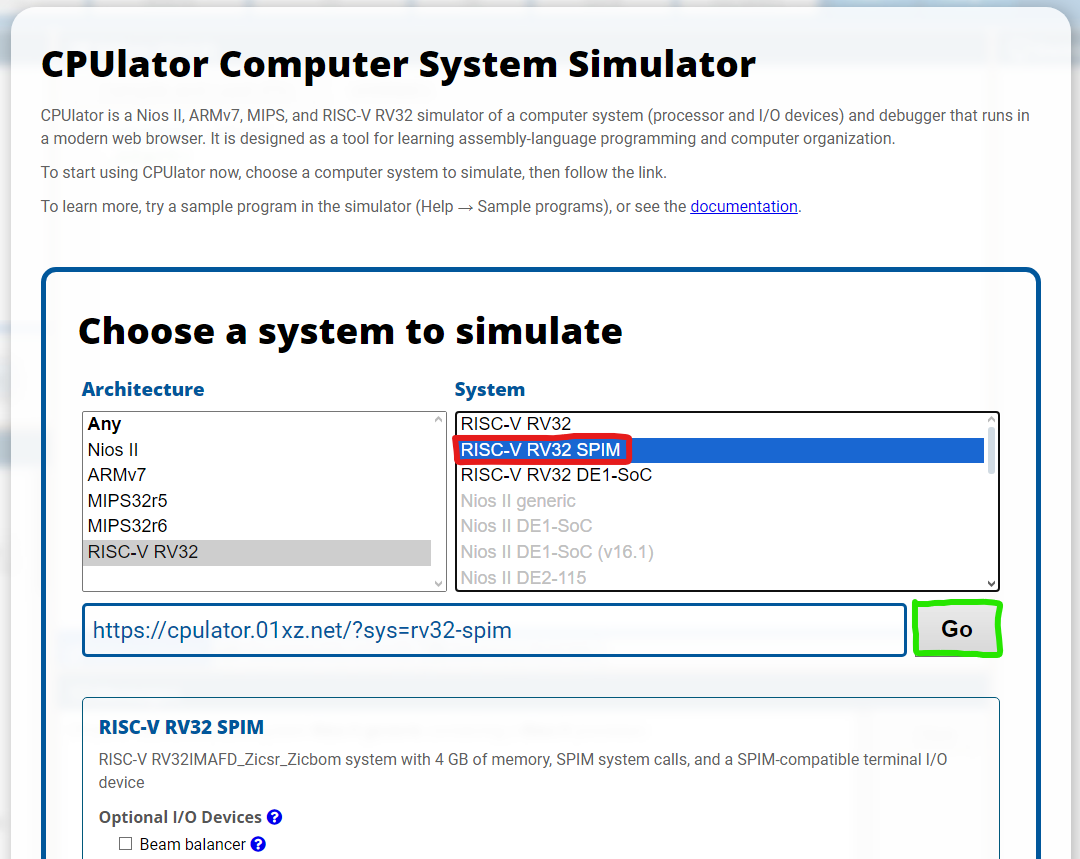
\includegraphics[width=0.5\linewidth]{spim}
    \caption{The RISC-V RV32 SPIM option}
\end{figure}

Once you click ``Go", you should see the same screen as in Figure 1.
Now, it's time to load the game itself onto CPUlator!

\subsection{Loading the game}

First, make sure you indeed see the same screen as in Figure 1.
Then, to load the game, look to the top of the interface at the blue bar.

\begin{figure}[ht]
    \centering
    
\includegraphics[width=0.7\linewidth]{bar}
    \caption{The blue bar near the top of the interface}
\end{figure}

Hover your mouse over the ``File" dropdown, and click the ``Open..." option.
Doing so should open a window where you can select a file.
Navigate to wherever you have the \texttt{game.s} file stored on your device, and select it.

\begin{figure}[ht]
    \centering
    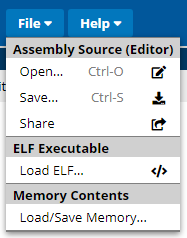
\includegraphics[width=0.2\linewidth]{dropdown}
    \caption{The dropdown menu when hovering over the ``File" option}
\end{figure}

The main screen should now contain lots of text. See Figure 7 for a reference.

\begin{figure}[ht]
    \centering
    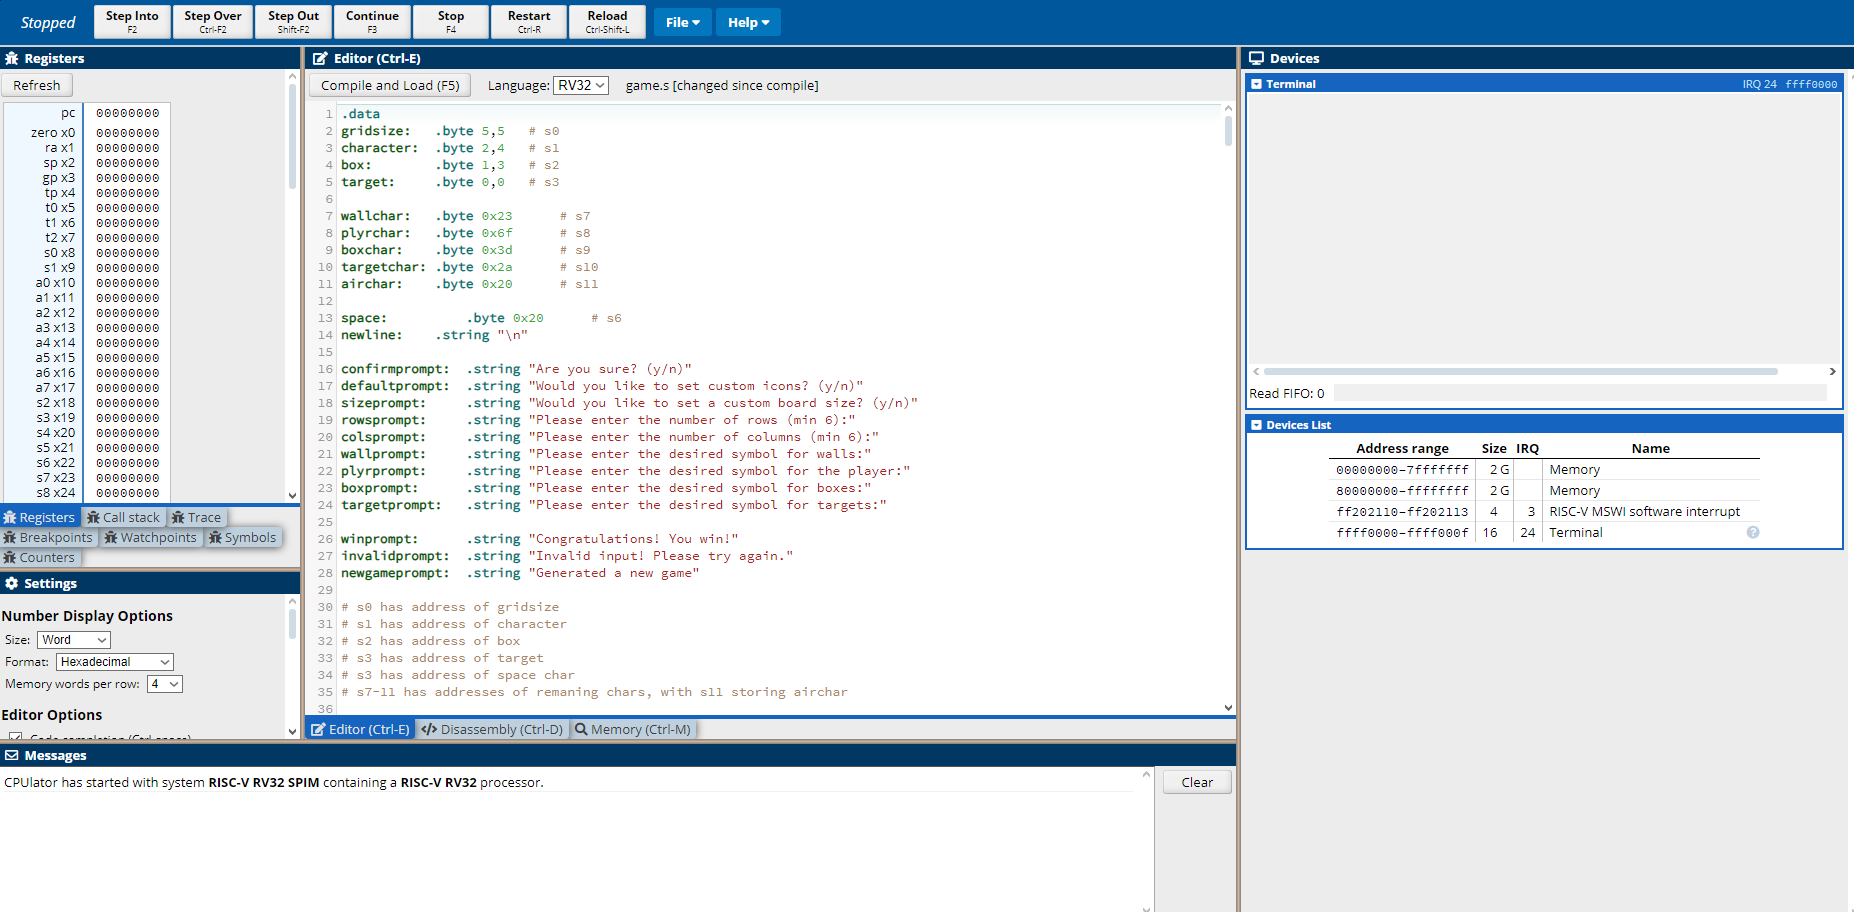
\includegraphics[width=0.8\linewidth]{filledscreen}
    \caption{The interface once the \texttt{game.s} file has been loaded}
\end{figure}

Congratulations - you've successfully loaded the game into CPUlator!

\subsection{Customizing your view}

Before continuing, you may want to take a moment to change the view a little.
Since this game is interacted with through the terminal, it would make sense that
the terminal be the largest portion of the interface.

Thankfully, CPUlator allows you to adjust and rescale the different segments of
the interface. If you hover your mouse over the line marked in red in Figure 8,
you can click and drag to adjust the terminal section to your liking.
See Figure 9 for an example of an adjusted window.

\begin{figure}[ht]
    \centering
    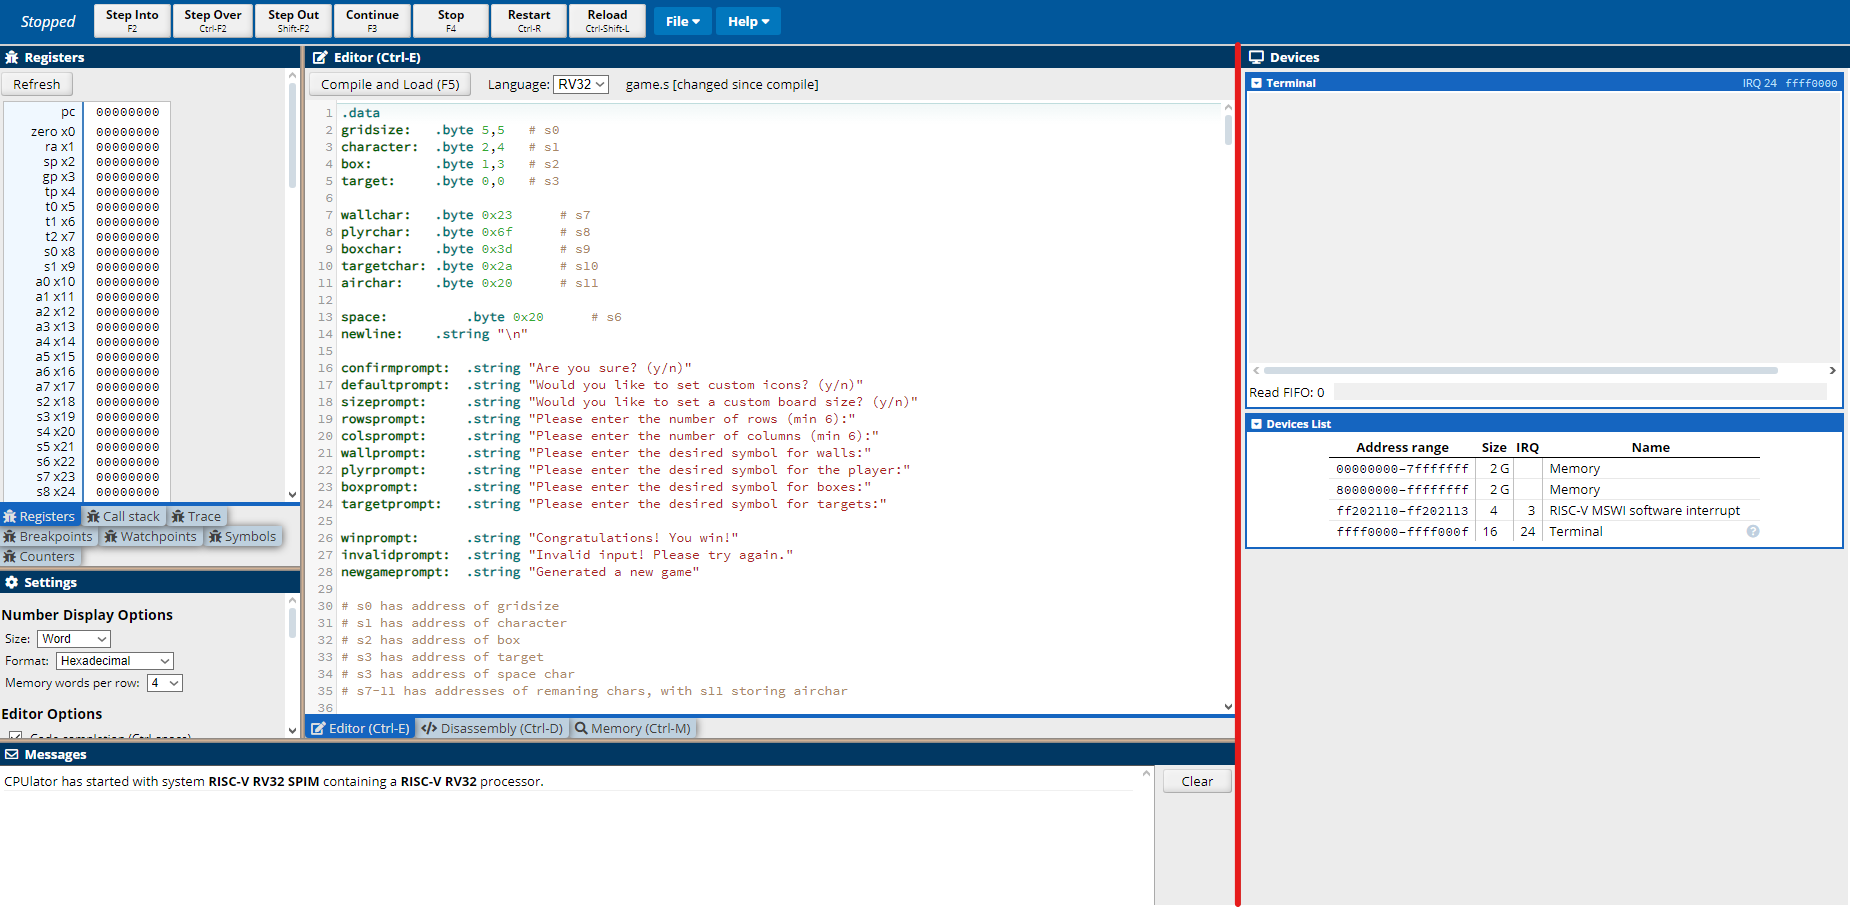
\includegraphics[width=0.8\linewidth]{adjustline}
    \caption{This line allows you to resize the terminal section}
\end{figure}

\begin{figure}[ht]
    \centering
    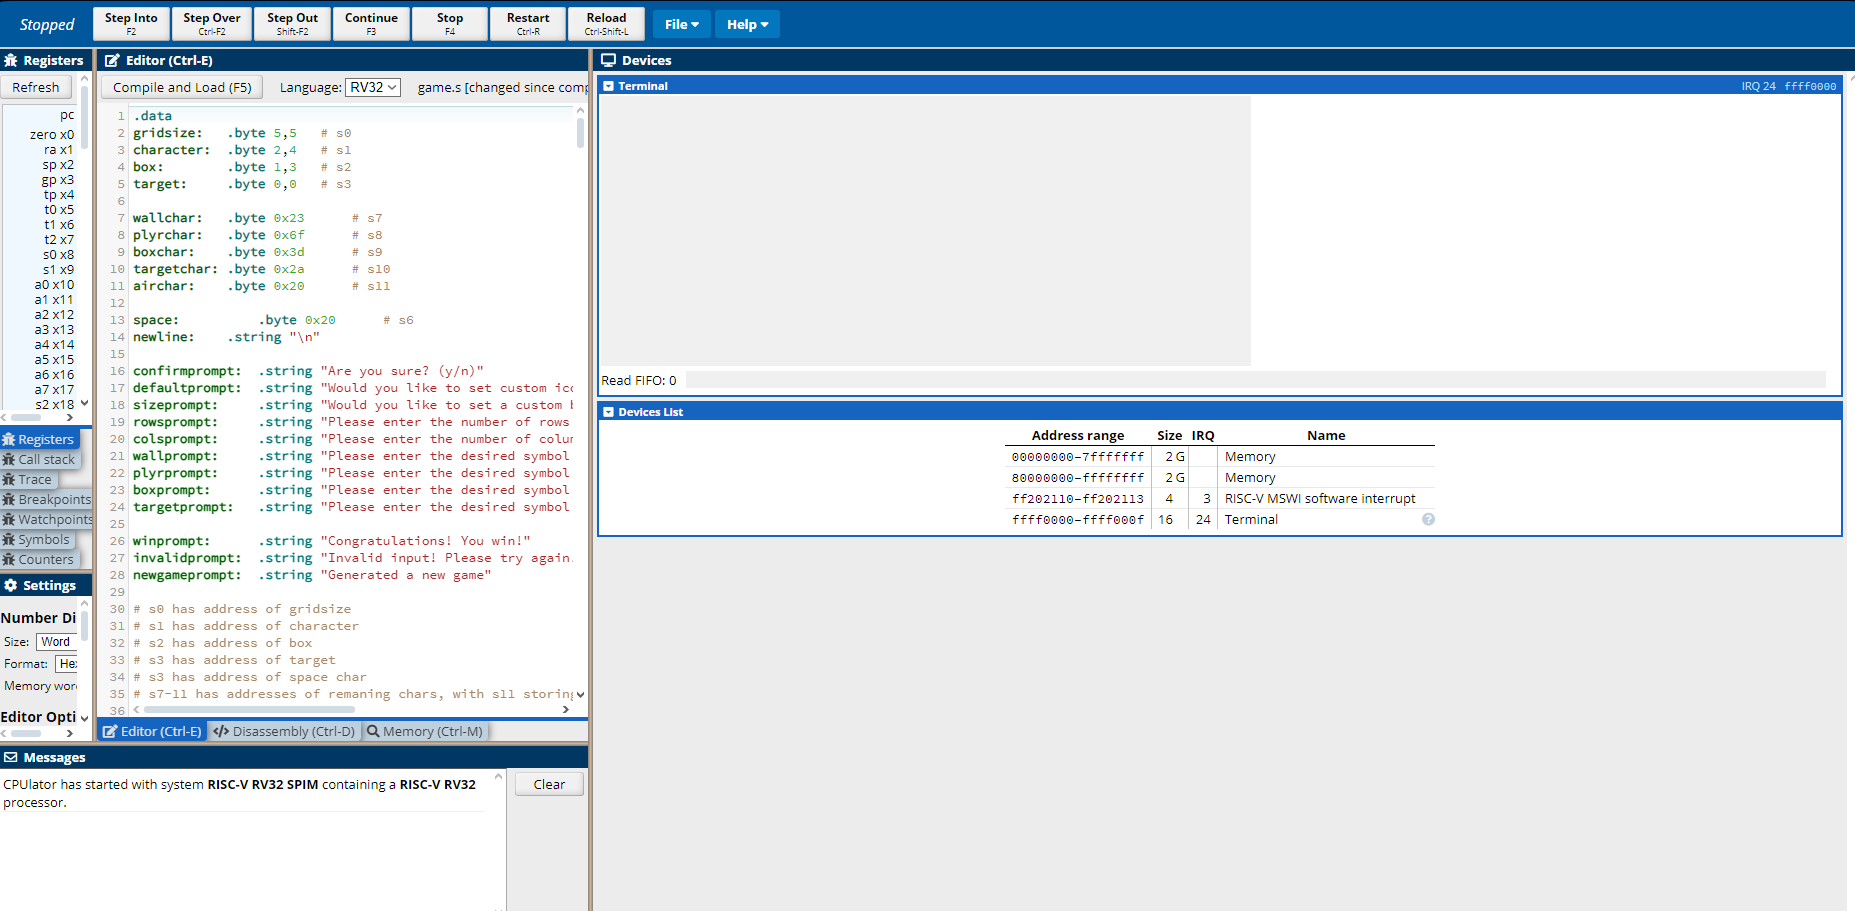
\includegraphics[width=0.8\linewidth]{adjusted}
    \caption{An example of a resized interface. You may prefer a different layout}
\end{figure}

Now that the terminal is front and center, we can \textit{really} play the game!

\newpage
\textcolor{white}{e}
\newpage
\section{Playing the game}
\subsection{Launching the game}

To start the game, you only have to click two buttons!

First, click the ``Compile and Load" button near the top left of the text-filled section.
The button is outlined in red in Figure 10 below.

\begin{figure}[ht]
    \centering
    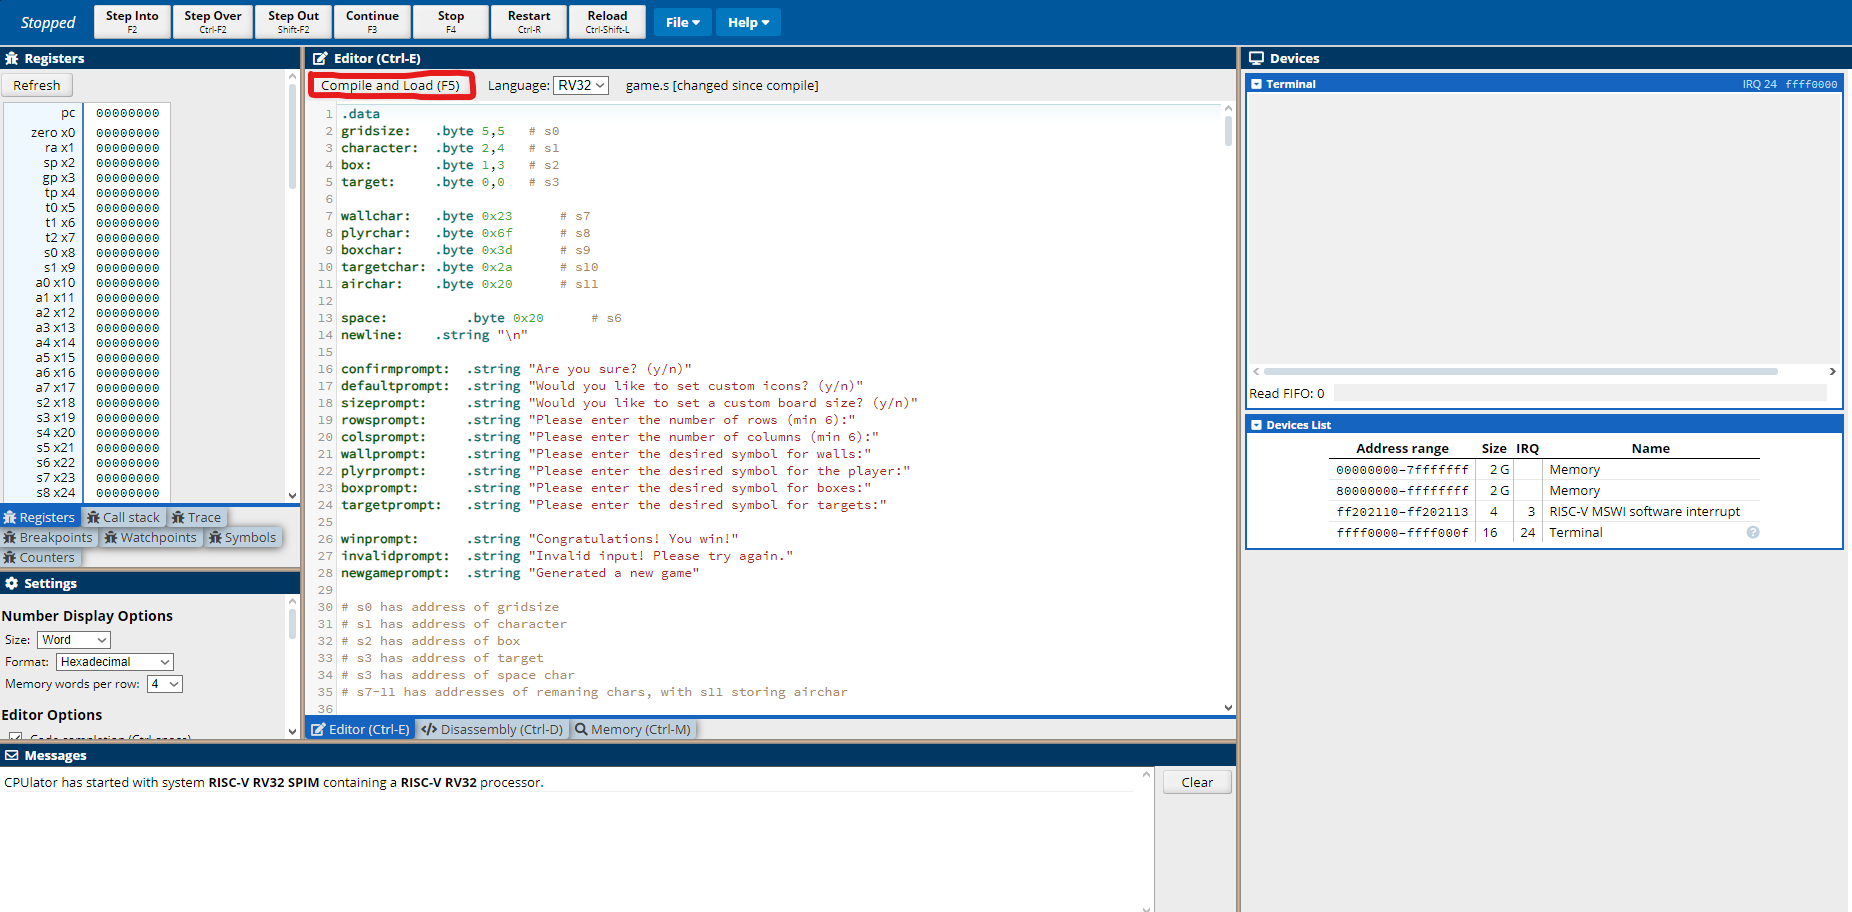
\includegraphics[width=0.8\linewidth]{compile}
    \caption{The Compile and Load button needs to be clicked first}
\end{figure}

Some of the windows might change, or text might appear. That's ok - all we have to do
is look back up at the blue bar and press the ``Continue" button.

\begin{figure}[ht]
    \centering
    
\includegraphics[width=0.8\linewidth]{continue}
    \caption{The Continue button gets the game running}
\end{figure}

At this point, the blue bar should turn green, and some text should have appeared on
the terminal. Great - you're ready to play Sokoban!

\subsection{Interaction and Controls}

Looking back at the terminal, you should see a prompt asking for a number of rows.
Note that you may have to click on the terminal window for your input to be registered.

Once you type a number and hit enter, it will also ask for a number of columns.
You may notice that the game enforces a minimum of 6 rows and columns.
This is done to stop the game from being \textit{too} easy, as well as for certain
technical reasons.

Once you've answered all the prompts, the terminal will begin printing out the game board
onto the terminal, as well as any relevant alerts/information. Here's what each symbol means:

\begin{itemize}
    \item A `\#' symbol is a wall. You cannot pass through these, and neither can the box.
    \item A `o' symbol is you, the player - you control this symbol!
    \item A `=' symbol is the box. Your goal is to move this to the target.
        \nopagebreak
    \item A `*' symbol is the target. Your goal is to move the box to here.
\end{itemize}

\newpage
\begin{figure}[ht]
    \centering
    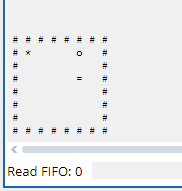
\includegraphics[width=0.2\linewidth]{sampleboard}
    \caption{An example of the game board}
\end{figure}

To move the character, the controls are as follows:

\begin{itemize}
    \item To move up, type `w'
    \item To move left, type `a'
    \item To move down, type `s'
    \item To move right, type `d'
    \item To generate a new game, type `r'
\end{itemize}

If any other character is submitted, the game will tell you in the terminal that the move is
invalid. This will also happen if you try to walk into or through a wall, or try to push the
box through a wall.

Once you've successfully moved the box to the target, the game will congratulate you before
terminating.

\begin{figure}[ht]
    \centering
    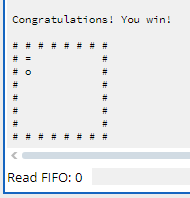
\includegraphics[width=0.2\linewidth]{victory}
    \caption{The congratulatory message upon victory}
\end{figure}

If you wish to play again, simply follow the steps in Section 4, and the game will start once again.

\newpage
\section{Gameplay Details}

(This section describes the game enhancements, which have not yet been implemented.)

\subsection{Competing with Friends}

One of the prompts upon starting the game asked for the number of players.
This version of Sokoban supports local multiplayer - you can take turns playing with your
friends!

Once you have taken your turn and completed the level, the board will reset back to its
initial state, and will prompt the next player to take their turn.

While each player takes their respective turn, the game will keep track of the number of moves
each player took in order to complete the level. Once everyone has taken their turn, a leaderboard
will be shown, ranking each player based on the number of moves taken to complete the level.

Currently, scores are not stored across sessions - if a new game is started, scores from the
previous game will not be considered on the leaderboard.

\subsection{Surrounded by Walls}

The board is also littered with more walls than just the border. Navigating these walls is part
of beating the game.

The game board is always generated with a valid solution - the game will never give you a board
which is impossible to beat.

The number of walls generated within the borders is calculated as follows:
\begin{gather*}
    W = \flr{\frac{LH}{4}} + 1 \\
    W = \trm{number of internal walls} \\
    L = \trm{length of the interior of the board} \\
    H = \trm{height of the interior of the board} \\
    \flr{x} = \trm{the floor function}
\end{gather*}

In other words, just over one-quarter of the interior of the board is composed of walls.

\end{document}
